%!TEX root = ./main.tex
\chapter{Introdução}
\label{introducao}

Simular numericamente a litosfera e astenosfera é um dos grandes desafios em dinâmica dos fluidos computacional. Ao mesmo tempo que a simulação numérica constitui um desafio matemático, a modelagem adequada da evolução de processos geodinâmicos, da reologia e da geometria das unidades litológicas constitui um desafio geofísico \citep{ranalli1995rheology,gerya2014precambrian}. 

No que diz respeito à matemática, o obstáculo está na solução das equações de conservação de massa, momento e energia, que não possuem soluções analíticas conhecidas. A diferença de viscosidade no interior do planeta Terra varia até 10 ordens de magnitude \citep[de $10^{16}$ à $10^{26}$ Pa s,][]{gerya-geodynamic-modelling}, enquanto a viscosidade de outros fluidos geofísicos varia menos do que uma ordem de magnitude. Somado à essa grande variação de viscosidade, a convecção no manto constitui um problema não-linear, especialmente em litosfera fria e rígida, o que dificulta a convergência de soluções numéricas \citep{gerya-geodynamic-modelling,zhong2015treatise}. 


% Essa diferença constitui um problema para convergência numérica, acentuado pelo comportamento não-linear do manto \citep{gery-geodynamic-modelling}. Além disso, convecção no manto constitui um problema não-linear, especialmente em litosfera fria e rígida, que, somado à grande variação de viscosidade, dificulta a convergência de soluções numéricas \citep{zhong2015treatise}. 

No contexto geofísico, a reprodução das iterações entre placas e a persistência de determinadas configurações ao longo de milhões de anos é fortemente dependente das suposições reológicas e geométricas iniciais, e devem corroborar com o conhecimento geofísico e geológico moderno \citep{schellart2007evolution,vanhunen2002}. Dessa forma, simulações numéricas buscam estabelecer vínculos entre os dados geológicos e geofísicos, quantificando os efeitos de diferentes processos ao longo do tempo geológico.

% Esse tipo de simulação lida com dificuldades não só matemáticas, mas que estão ligadas à evolução dos processos geodinâmicos, da reologia e da geometria das unidades litológicas \citep{ranalli1995rheology,gerya2014precambrian}, tudo isso na escala de milhões de anos. E todos esses fatores devem funcionar juntos para reproduzir as interações observadas entre placas e garantir a persistência de determinadas configurações ao longo do tempo \citep{schellart2007evolution,vanhunen2002}.

% E essa dinâmica é sensível a uma série de fatores, que influenciam tanto as interações observadas entre placas quanto a persistência de determinadas configurações ao longo do tempo, tudo isso na escala de milhões de anos \citep{schellart2007evolution,vanhunen2002}.

% O desafio fica ainda mais evidente quando analisamos 

Comparadas às simulações de regiões onde há convecção somente na astenosfera \citep[modelos do tipo Rayleigh-Taylor,][]{gerya-geodynamic-modelling}, simulações de placas em subdução são ainda mais desafiadoras, à medida que lidam com a interação entre placas, dificuldade ligadas à reologia atual e sua evolução, e até mesmo aos mecanismos responsáveis pelo início da subdução, que não apresenta consenso dentro da comunidade científica. 
%Isso dificulta ainda mais a simulação de zonas de subdução do que em regiões onde há convecção somente na astenosfera, modelos do tipo Rayleigh-Taylor \citep{gerya-geodynamic-modelling}.

Para essa etapa do projeto, pretendo lidar com esses desafios e simular numericamente a subdução da placa de Nazca sob a placa da América do Sul para geometrias sintéticas, considerando uma reologia apropriada, e destacar os parâmetros que controlam a subdução como a observamos com a sismologia hoje.
%O presente trabalho pretende lidar com todos esses desafios e simular numericamente a subdução da placa de Nazca sob a placa da América do Sul, considerando uma reologia apropriada, e quantificar a contribuição da subdução da Dorsal de Nazca na evolução do arco de Fitzcarrald, no oeste Amazônico.

\section{Dorsais oceânicas}

%Dorsais oceânicas são regiões no planeta onde litosfera oceânica é continuamente produzida. 

% À medida que duas placas oceânicas se afastam, material de origem mantélica é expelido de seu eixo de afastamento. Esse material dá forma à uma dorsal e produz nova litosfera ao depositar basalto no assoalho oceânico \citep{turcotte2002geodynamics}. Em termos relativos, quanto mais próximo da dorsal, mais fina, jovem e quente é a litosfera oceânica. 
%Quando a dorsal deixa de produzir litosfera nova, ela é denominada de dorsal fóssil.

No contexto da tectônica de placas, em um limite divergente há produção de litosfera oceânica a partir de basalto oriundo do manto astenosférico, \textit{mid ocean ridge basalt} (MORB). Esse basalto é expelido dando forma à dorsais e produz nova litosfera oceânica ao ser depositado no assoalho oceânico \citep{turcotte2002geodynamics}. As forças resultantes na região de elevação topográfica compõem um força de empurrão, \textit{ridge-push}, que promove o afastamento axial das placas jovens e é uma das principais forças motrizes da tectônica de placas \citep{allen2013basin}. Ao se afastarem, as litosferas esfriam, espessam e tornam-se mais densas por contração térmica. Em termos relativos, quanto mais próximo da dorsal, mais fina, jovem e quente é a litosfera oceânica.

Um outro tipo de dorsal tem origem geralmente associada aos efeitos de um \textit{hotspot} estacionário sob uma litosfera móvel \citep{vanhunen2002,vogt1973}. Esse tipo de dorsal é classificada como \emph{assísmica} e, além de não apresentar sismicidade importante, possui uma crosta excessivamente espessa e não apresenta vulcanismo (e consequentemente não produz nova litosfera oceânica). 

\section{Zonas de subdução}

Zonas de subdução, por sua vez, são regiões onde placas litosféricas (relativamente espessas, velhas e frias) descendem para o interior do manto terrestre. Ao passo que a litosfera evolui, sua densidade e sua espessura aumentam em decorrência do resfriamento por condução e da incorporação de material do manto à sua base que, após atingir um limite, mergulham em direção ao interior do planeta \citep{turcotte2002geodynamics}. 

Como a litosfera oceânica pode ser entendida como uma placa elástica, sua porção em subdução puxa em direção à trincheira o restante da placa, o que constitui a principal força motriz da tectônica de placas, denominado de \textit{slab-pull} ou \textit{trench-pull}, e cuja magnitude pode ser até $10$ vezes maior do que o \textit{ridge-push} mencionando anteriormente \citep{allen2013basin}. 

A trincheira, por sua vez, forma-se com o arqueamento da placa em subdução e sua morfologia e convexidade dependem da reologia da placa \citep{turcotte2002geodynamics}. Essa feição, no entanto, não é estacionária, ocorrendo migração da trincheira na direção oposta da subdução em todos os referenciais. Esse deslocamento tem implicações na extensão do retroarco, entre o orógeno e a bacia de ante-país, e também no padrão de convecção geral do manto superior, já que mudanças na área da placa em subdução afetam o transporte de calor e o vigor de convecção no manto \citep{becker2009review}. Durante os últimos $50$ milhões de anos, por exemplo, estima-se que a trincheira Andina, resultado da subdução da placa de Nazca sob a placa da América do Sul, recuou mais de $1000$ km com uma taxa média superior à $20$ mm/ano \citep{schellart2007evolution}.

A subdução de litosfera também não ocorre de maneira uniforme. Porções de litosfera oceânica subduzem com ângulos e velocidades diferentes em virtude de sua geometria complexa, da idade e da temperatura ao longo da mesma zona de subdução \citep{barazangi1976spatial,cahill1992seismicity,muller2008age}. Na América do Sul, por exemplo, há regiões onde a subdução é ``normal'' \citep{barazangi1976spatial,cahill1992seismicity}, regiões com subdução de dorsal assísmica \citep{espurt2007nazca,manea2012chilean,gutscher1999tectonic,alvarado2009flat} e uma região onde a placa em subdução apresenta possível rompimento \citep{barazangi1976spatial}. Em cada uma dessas regiões, a placa descendente vai apresentar uma trajetória diferente com efeitos diretos na placa sobrejacente. Um exemplo desses efeitos é a evolução do Arco de Fitzcarrald no oeste Amazônico, resultado da subdução da placa de Nazca com baixo ângulo de mergulho \citep{espurt2007nazca}.

% A subdução de litosfera também não ocorre de modo uniforme. Porções de litosfera oceânica subduzem com ângulos e velocidades diferentes em virtude de sua geometria complexa, da idade e da temperatura ao longo da mesma zona de subdução \citep{muller2008age}. Na placa de Nazca, por exemplo, há regiões onde ocorre subdução de dorsal assísmica, que apresenta crosta oceânica espessa e litosfera relativamente fina, como ilustra esquematicamente a figura \ref{ridge-subduction}.% mostra um esquema da subdução de uma litosfera oceânica com dorsal assísmica e cuja direção do movimento da placa é perpendicular ao eixo da trincheira.

\begin{figure}[htb]
  \begin{center}
    \includegraphics[width=0.9 \columnwidth]{fig/ridge-subduction.png}
  	\caption{\label{ridge-subduction}Esquema de uma litosfera oceânica com uma dorsal assísmica que subduz sob uma litosfera continental. As setas indicam a direção do movimento da placa, que é perpendicular ao eixo da trincheira.}
  \end{center}
\end{figure}

% A figura \ref{ridge-subduction} ilustra o espessamento da crosta oceânica e afinamento litosférico sob a dorsal assísmica, que é típico desse padrão de subdução.

Uma placa oferece maior ou menor resistência à curvatura de acordo com sua velocidade de subdução, densidade e espessura. Uma litosfera oceânica com maior rigidez flexural, por exemplo, vai resistir a mudanças de trajetória localmente, o que significa que seu percurso deve ser menos perturbado se comparado ao de uma placa com menor rigidez flexural \citep{assuncao2019}.
% Velocidade de subdução, densidade e espessura afetam diretamente a trajetória de uma placa em subsuperfície \citep{assuncao2019}, consequência de uma litosfera oceânica com maior rigidez flexural, ou seja, que oferece maior resistência à curvatura.
% Outro exemplo é o caso de uma litosfera mais velha, e densa, que subduz com um ângulo maior do que uma litosfera mais jovem, e relativamente menos densa.
%Outro exemplo é o caso de uma litosfera mais velha, e densa, que vai possuir uma velocidade de subdução maior do que uma litosfera mais jovem, e fina. 

Outros fatores também são determinantes na evolução do ângulo de subdução e na trajetória da placa em subdução, tais como o recuo da trincheira, sucção hidrodinâmica, composição e estrutura térmica da litosfera, e subdução de dorsal assísmica \citep{schellart2007evolution,bishop2017,antonijevic2015}. Faz parte deste trabalho entender melhor esse fatores e verificar quais deles são necessários e/ou suficientes para o caso de estudo.

A litosfera descendente também tem papel fundamental na ocorrência dos fenômenos geológicos observados na placa sobrejacente que, de modo geral, atua como moduladora da perda de calor do planeta, regula convecção do manto terrestre, estabelece a localização de terremotos e vulcões, possibilita a ocorrência da tectônica de placas e, portanto, tem grande impacto nos processos formadores da topografia \citep{zhong2015treatise,mooney2015treatise}. 

No que diz respeito ao padrão de convecção astenosférico no tempo geológico, a geometria da placa em subdução afeta diretamente o padrão de escoamento do manto, favorecendo ou impedindo padrões de convecção que, por sua vez, interagem com a própria placa e com a litosfera sobrejacente.

A figura \ref{fig:esquema-subducao} mostra um esquema de um padrão de convecção em região de subdução de litosfera oceânica sob litosfera continental. Na imagem, material quente e de densidade relativamente baixa ascende sob a região de dorsal e, enquanto esfria em contato com a base da litosfera, flui na direção da trincheira oceânica acompanhando a geometria da base da placa e descende para o interior do planeta acompanhando a geometria da litosfera em subdução. Na porção sobrejacente à placa em subdução, o padrão de convecção converge para a cunha mantélica e descende após resfriar e se tornar mais denso, acompanhando a geometria do topo da placa descendente. As outras regiões indicadas com um símbolo de interrogação são regiões de indeterminação.
    
\begin{figure}
    \centering
    \includegraphics[width=\textwidth]{fig/esquema-subducao.png}
    \caption{Esquema simplificado do padrão de convecção em região de subdução de litosfera oceânica sob litosfera continental. A litosfera lubrificante faz parte da litosfera continental, mas apresenta uma reologia que contribui para facilitar a subdução.}
    \label{fig:esquema-subducao}
\end{figure}

Outros padrões de convecção vão agir, por exemplo, sobre o afinamento e espessamento litosférico, ocorrência de vulcanismo, criação de nova litosfera oceânica e crosta continental, topografia dinâmica e forças de sucção hidrodinâmica \citep{allen2013basin,braun2010many,schepers_etal2017,stern2002subduction}.

\section{Região de estudo}
\label{areaDeEstudo}

% O que pretende-se entender nesta primeira etapa do doutorado é o que seria necessário para simular numericamente o manto e a litosfera fria na região da Dorsal de Nazca e do arco de Fitzcarrald, onde a placa de Nazca subduz sob a placa da América do Sul. A Dorsal de Nazca não apresenta vulcanismo, tem uma crosta bastante espessa e é assísmica.

%A figura \ref{slab2} mostra a porção da placa de Nazca que subduz  sob a placa da América do Sul \citep[modelo Slab2,][]{hayes2018slab2}. À esquerda (figura \ref{slab2}a) é mostrado o mapa do ângulo de mergulho da placa de Nazca ao longo da zona de subdução e na imagem à direira (figura \ref{slab2}b) o mapa de sua profundidade é apresentado. Entre as latitudes $-2,5$º e $-15,0$º e depois entre $-25,0$º e $-35,0$º, o ângulo e a profundidade da placa de Nazca se mantêm pequeno ($<5$º) e razoavelmente constante (entre $80$ e $100$ km), respectivamente. Essas características compõem uma subdução do tipo \textit{flatslab}, onde a placa pode permanecer sub-horizontal por centenas de quilômetros antes de mergulhar com um ângulo de subdução maior. 

A placa de Nazca move-se para leste e subduz sob a placa da América do Sul, como ilustram as imagens da figura \ref{slab2} \citep[modelo Slab2,][]{hayes2018slab2}. Ao longo da zona subdução, a figura \ref{slab2dip} apresenta o ângulo de mergulho da placa de Nazca e a figura \ref{slab2dep} apresenta a profundidade de seu topo.

\begin{figure}
  \centering

  \subfloat[][Mapa do ângulo de mergulho da placa de Nazca.]{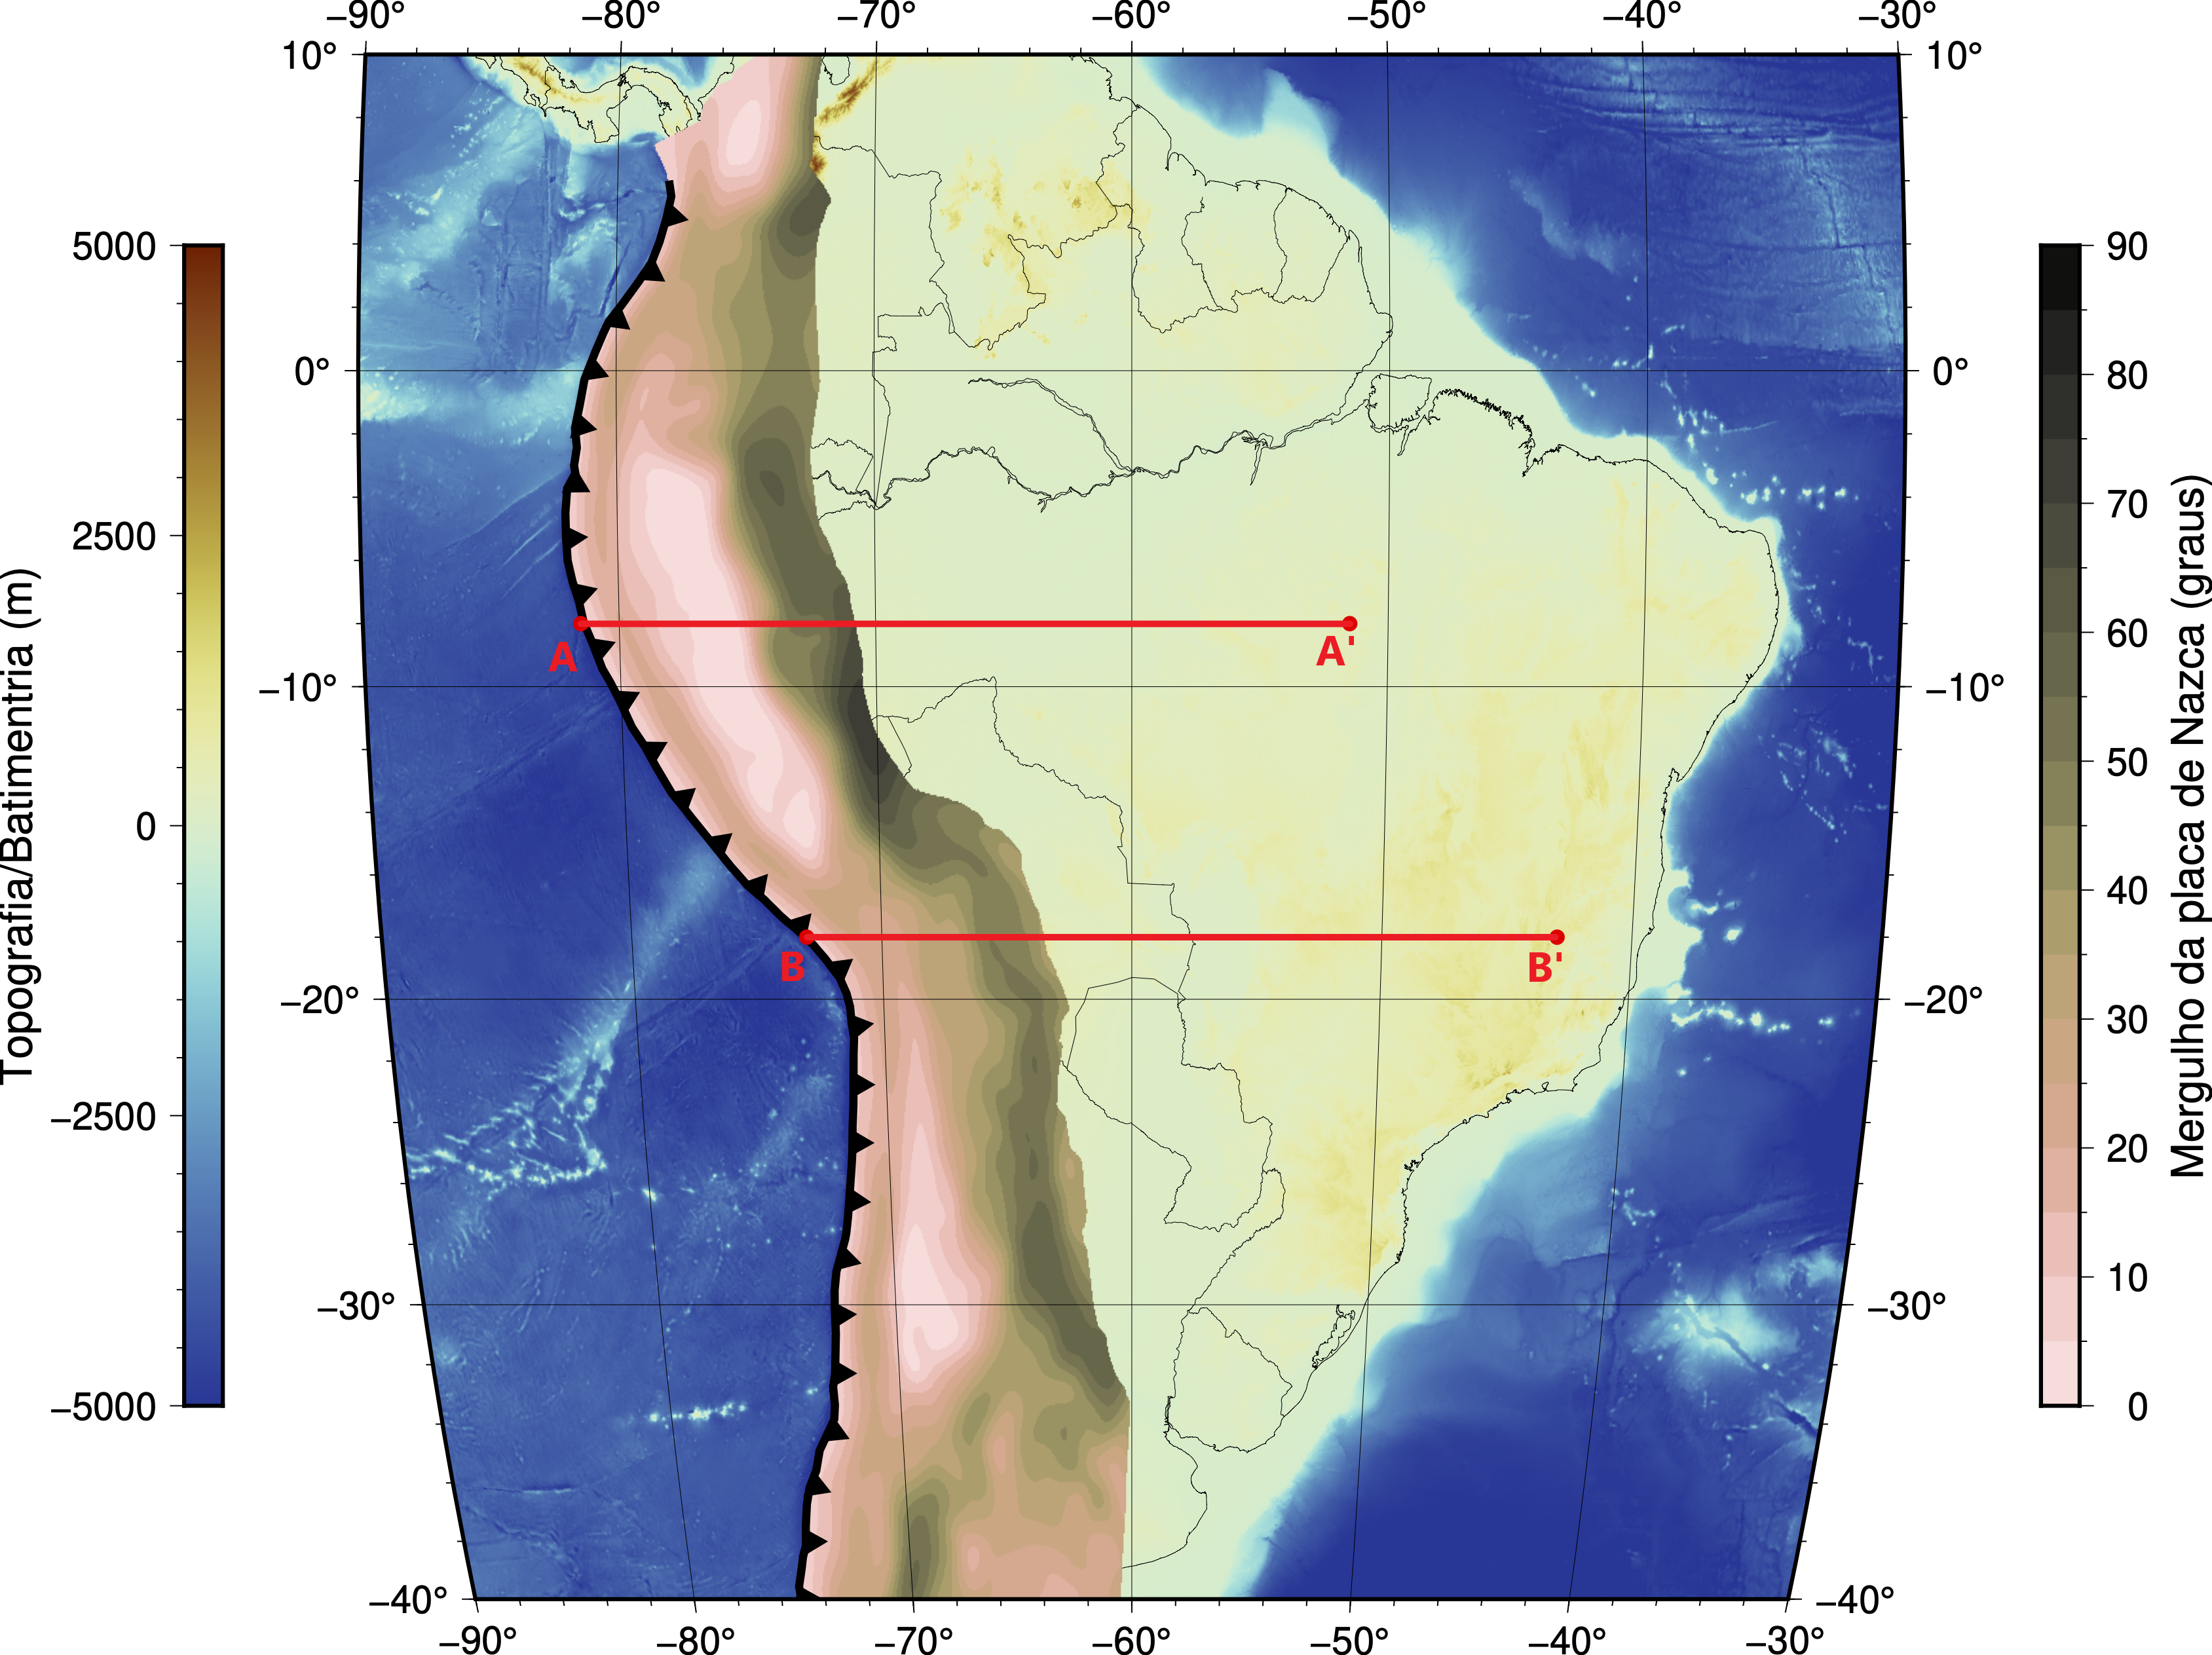
\includegraphics[width=0.83\columnwidth]{fig/slab2dip.png}\label{slab2dip}}

  \vspace{0.5cm}

  \subfloat[][Mapa da profundidade do topo da placa de Nazca.]{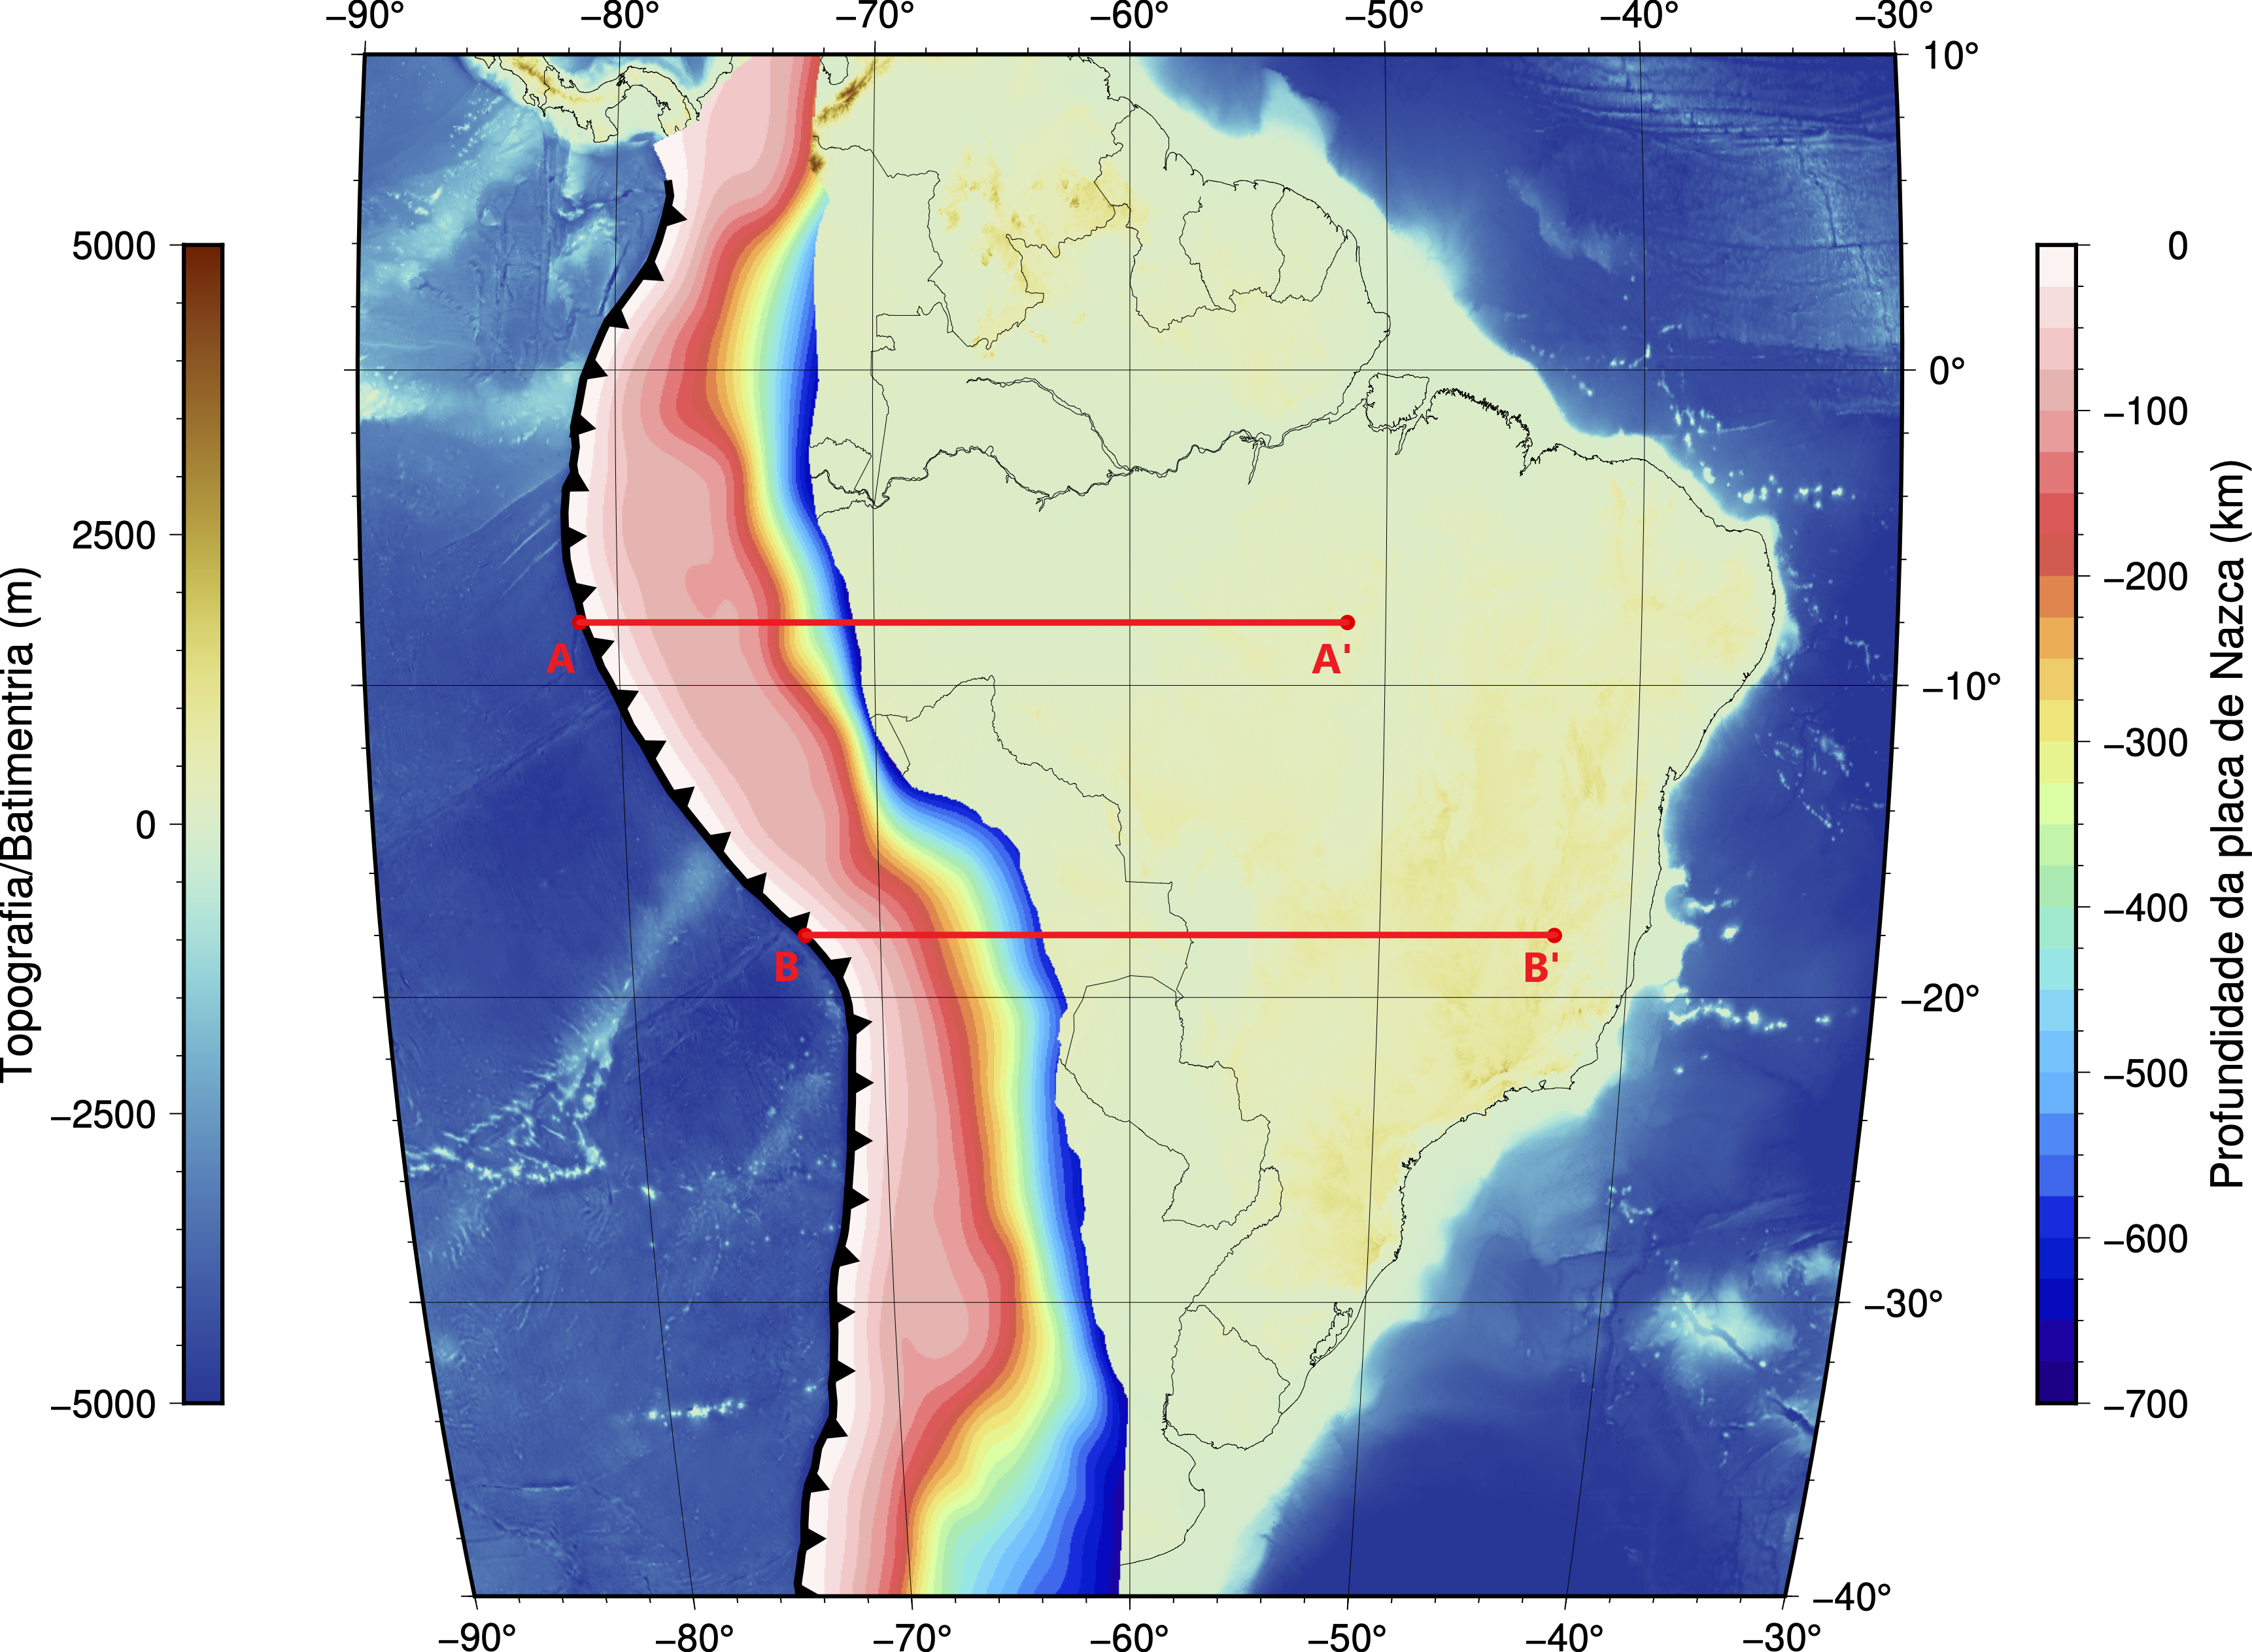
\includegraphics[width=0.83\columnwidth]{fig/slab2dep.png}\label{slab2dep}}
    
  \caption{Mapas do ângulo de mergulho e da superfície superior da placa de Nazca. Dados extraídos do modelo Slab2 \citep{hayes2018slab2}.}
  \label{slab2}
    
\end{figure}

Entre as latitudes $-2,5$º e $-15,0$º e depois entre $-25,0$º e $-32,0$º, o ângulo de subdução mantém-se pequeno ($<5$º) e a profundidade da placa é razoavelmente constante (entre $80$ e $100$ km). Esses segmentos sub-horizontais (\textit{flatslabs}) estendem-se por centenas de quilômetros antes de mergulharem com um ângulo de subdução maior. A título de comparação, a figura \ref{tomografias} apresenta quatro modelos tomográficos independentes \citep{obayashi2013pwavetomography,fukao2013subductedslabs,simmons2012pwavetomography,amaru2007global,lu2019seismictomography} para dois perfis marcados na figura \ref{slab2}, com o perfil A-A' (figura \ref{tomografiaPerfilA}) e o perfil B-B' (figura \ref{tomografiaPerfilB}) dentro e fora do trecho \textit{flatslab}, respectivamente. 

\begin{figure}
  \centering

  \subfloat[][Tomografia do perfil A-A', de latitude $-8.0$ e longitudes de $-73.0$ à $-43.0$.]{\includegraphics[trim={18cm 72cm 18cm 2cm}, clip, width=0.40\columnwidth]{fig/profileA.png}\label{tomografiaPerfilA}}\hspace{0.5cm}
  \subfloat[][Tomografia do perfil B-B', de latitude $-18.0$ e longitudes de $-81.5$ à $-51.5$.]{\includegraphics[trim={18cm 72cm 18cm 2cm}, clip, width=0.40\columnwidth]{fig/profileB.png}\label{tomografiaPerfilB}}
    
  \caption{Modelos tomográficos dos perfis A-A' e B-B' da figura \ref{slab2}. Os modelos GAP-P4 \citep{obayashi2013pwavetomography,fukao2013subductedslabs}, LLNL\_G3Dv3 \citep{simmons2012pwavetomography} e UU-P07 \citep{amaru2007global} são de ondas P e o modelo TX2019slab-S \citep{lu2019seismictomography} é de onda S.}
  \label{tomografias}
\end{figure}

Para o perfil A-A' e até $660$ km de profundidade (figura \ref{tomografiaPerfilA}) é possível perceber que a anomalia positiva de velocidade acompanha a geometria sub-horizontal da placa de Nazca apresentada pelo Slab2 na figura \ref{slab2}, com destaque para os modelos UU-P07 e TX2019slab-S que apresentam uma anomalia positiva de velocidade que definem bem a placa descendente. 

A anomalia positiva de velocidade no perfil B-B' até $660$ km de profundidade (figura \ref{tomografiaPerfilB}) sugere um ângulo de subdução maior, sem sub-horizontalização, e também concorda com o modelo Slab2 da figura \ref{slab2}. Vale ressaltar que o perfil B-B' passou por episódios de \textit{flatslab} \citep{ramos2009andean}, mas que a geometria atual da placa até $400$ km de profundidade, observada nos perfis tomográficos, é distinta do que se observa no perfil A-A' na figura \ref{tomografiaPerfilA}.

No perfil fora da região de \textit{flatslab}, a placa de Nazca apresenta uma região ampla de anomalia positiva entre $660$ e $1000$ km, onde deve ocorrer espessamento da placa, e mantém-se contínua até $1500$ km de profundidade no modelo LLNL\_G3Dv3 e passa dos $2000$ km nos demais modelos.

No perfil dentro da região de \textit{flatslab}, a placa também apresenta uma região ampla de anomalia positiva entre $660$ e $1000$ km, mantém-se contínua até cerca de $1500$ km de profundidade, mas apresenta uma anomalia que sugere sub-horizontalização próximo à $1000$ km.

% Contida na região de \textit{flatslab} mais setentrional da figura \ref{slab2}, a região de estudo é mostrada na figura \ref{nazca-ridge}, onde a dorsal de Nazca subduz sob a margem Peruviana. Um dos efeitos dessa subdução sub-horizontal é a deformação da região de ante-país na qual está localizado o arco de Fitzcarrald, a 750 km da margem oeste da América do Sul, no oeste da bacia Amazônica \citep{espurt2007nazca}.

% \begin{figure}[htb]
%   \begin{center}
%     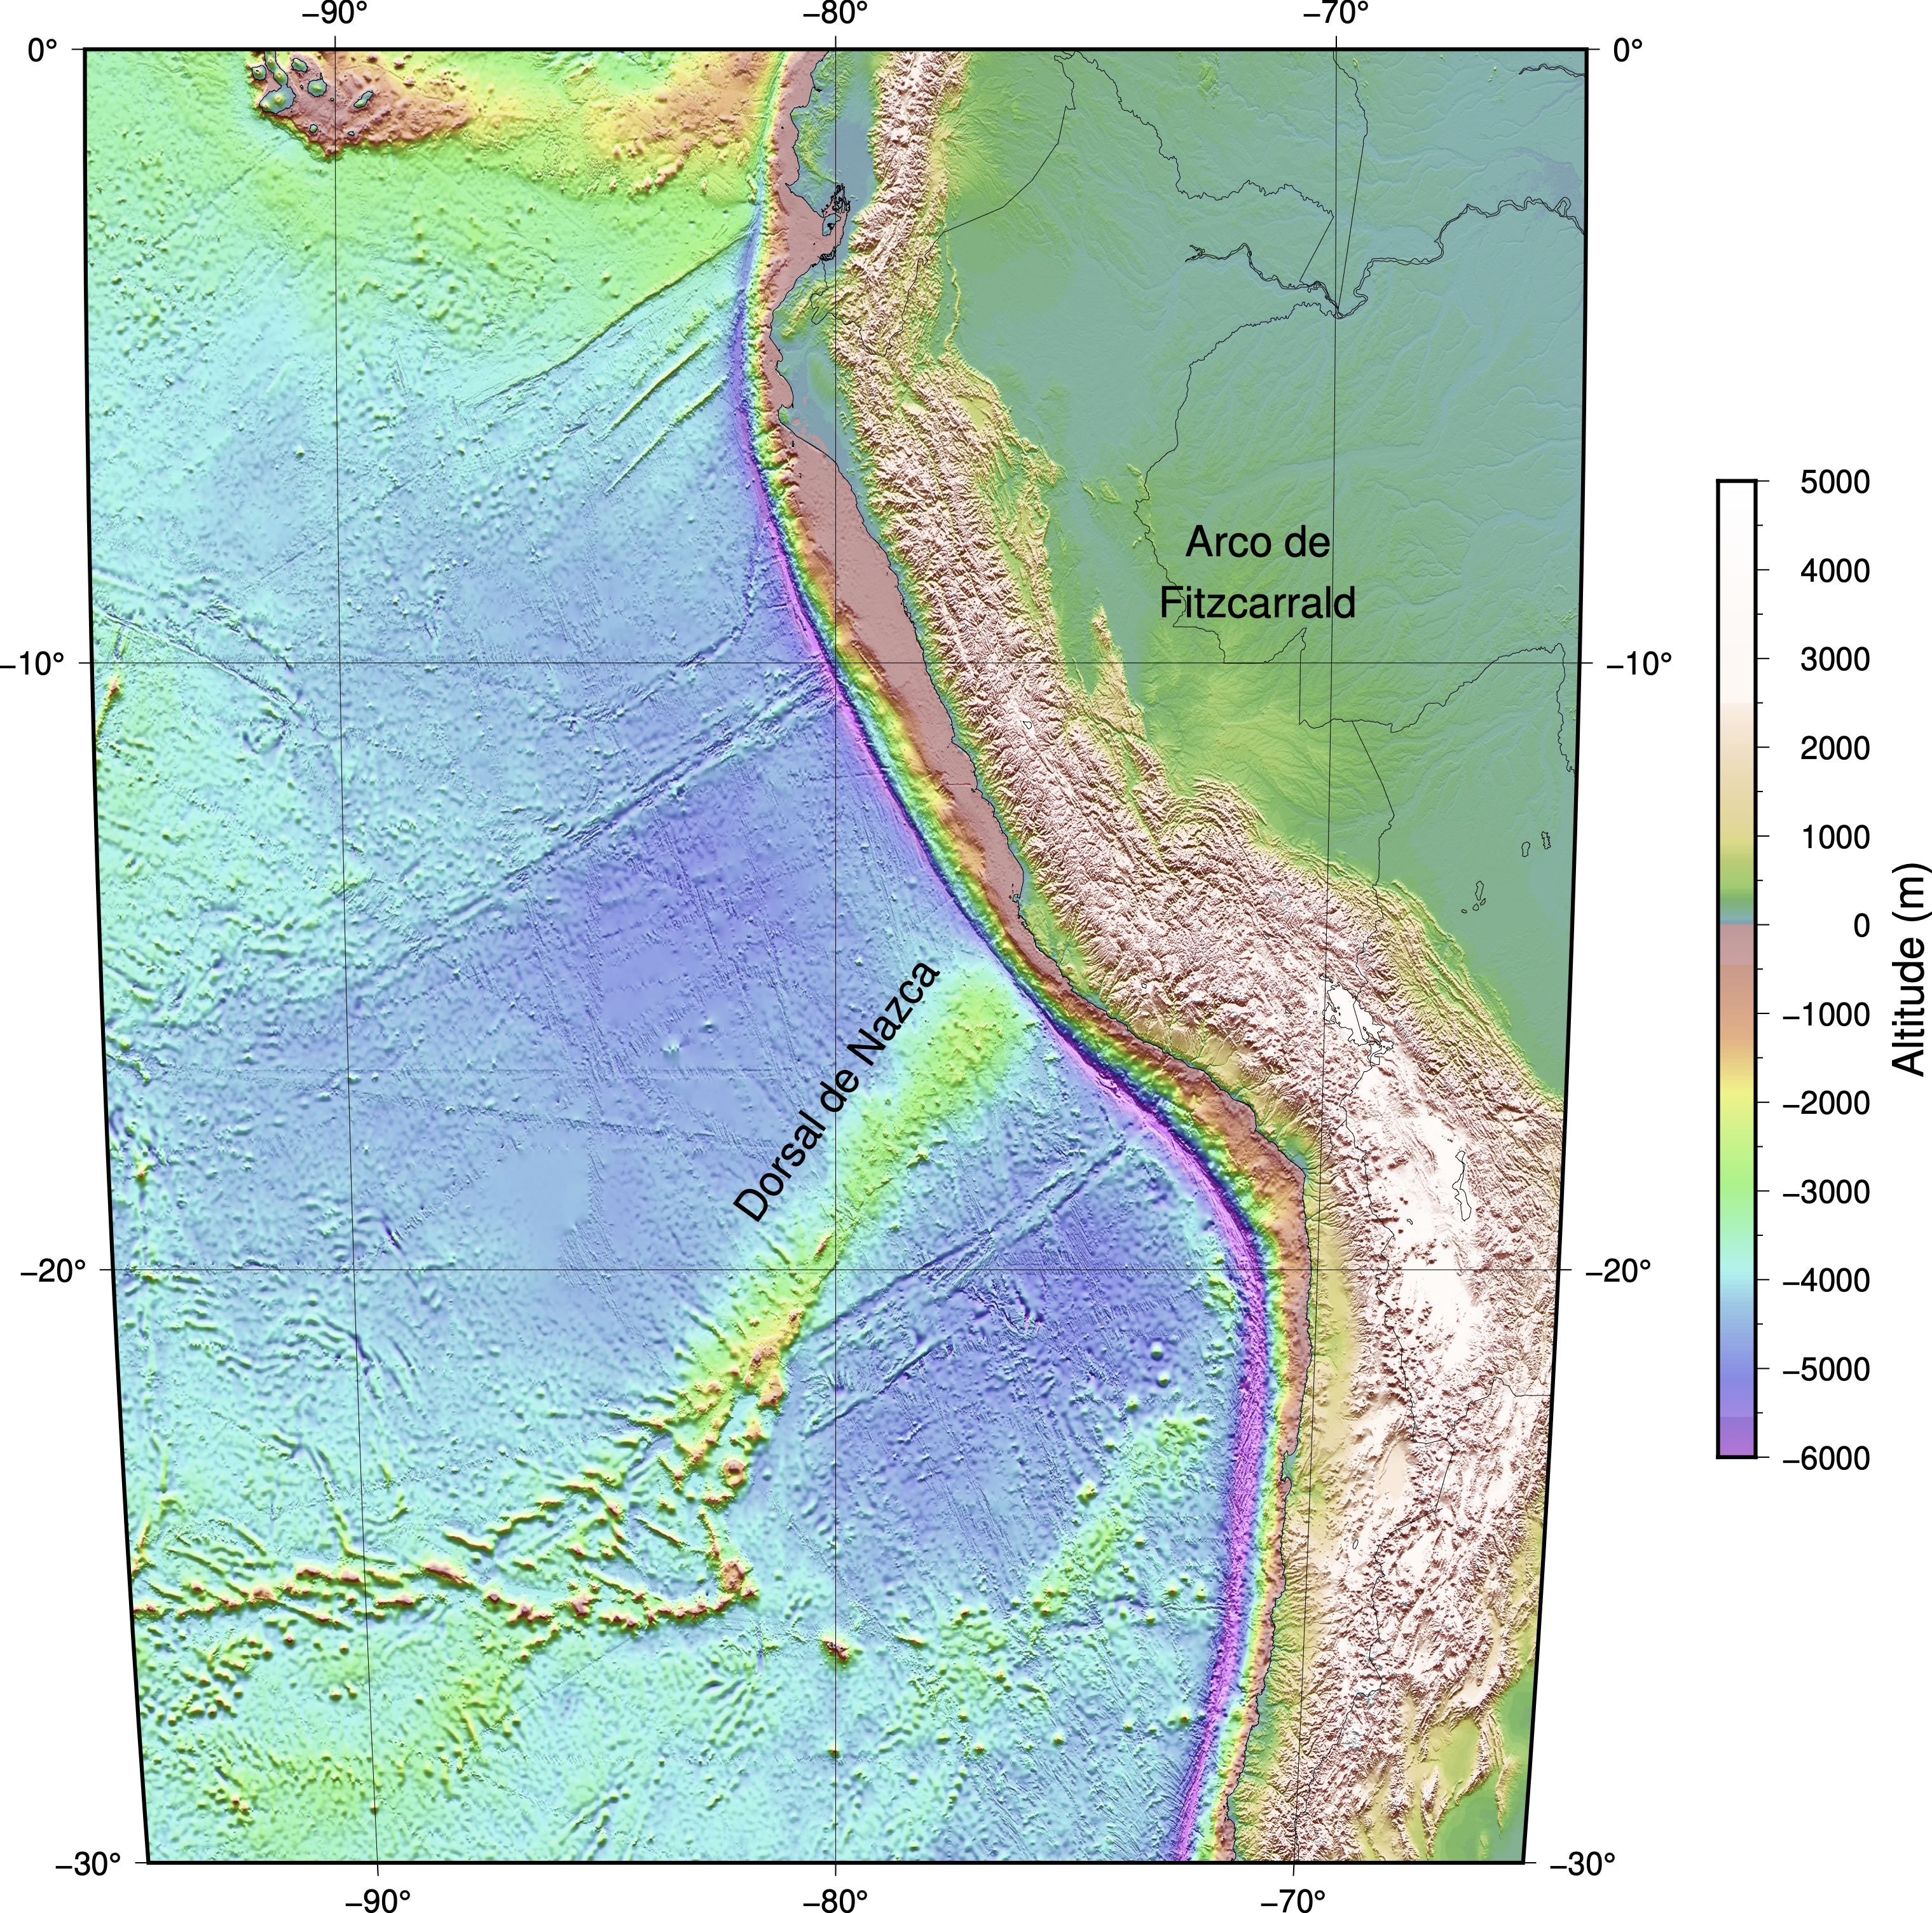
\includegraphics[width=0.8 \columnwidth]{fig/nazca.png}
%   	\caption{\label{nazca-ridge} Localização da Dorsal de Nazca e do arco de Fitzcarrald. Dados de elevação de \cite{tozer2019}.}
%   \end{center}
% \end{figure}

% A Dorsal de Nazca é uma dorsal assísmica e dados sismológicos mostram que o \textit{flatslab} é relativamente mais raso ao longo do seu eixo e está afundando, rasgando e reiniciando subdução normal na porção noroeste \citep{antonijevic2015}.

% % On the basis of our observations, we propose a conceptual model for the temporal evolution of the Peruvian flat slab in which the flat slab forms because of the combined effects of trench retreat along the Peruvian plate boundary, suction, and ridge subduction. We find that while the ridge is necessary but not sufficient for the formation of the flat slab, its removal is sufficient for the flat slab to fail. This provides new constraints on our understanding of the processes controlling the beginning and end of the Laramide orogeny and other putative episodes of flat-slab subduction.

% Simular numericamente a região de estudo corresponde a simular o trecho de \textit{flatslab} que contém a dorsal assísmica. Na primeira parte do doutorado farei simulações sintéticas, buscando simplificar a geometria da dorsal assísmica em subdução e entender a influência dos parâmetros realizando testes de sensibilidade. A segunda parte do doutorado vai simular a subdução na região usando dados geofísicos e geológicos, tais como os modelos de \cite{hayes2018slab2} e \cite{pasyanos2014litho1}, e dessa forma entender a influência da subdução sub-horizontal da Dorsal de Nazca na evolução do interior do continente Sul-Americano. 

% Uma das principais razões da estabilidade do trecho \textit{flatslab} na região de estudo é a sua reologia. À medida que a temperatura da rocha aumenta para um valor próximo da temperatura de fusão, há mobilidade suficiente dentro da estrutura cristalina para haver movimentação dos átomos por arrasto \citep{turcotte2002geodynamics}. O fluxo resultante é um dos agentes que controlam a trajetória da placa em subdução, impedindo ou permitindo que determinadas geometrias perdurem \citep{assuncao2019,schellart2007evolution}.

% Conforme a placa em subdução passa por processos de metamorfismo e mudança de fase, sua densidade aumenta e a interação da placa com o manto circundante fica mais complexa. A figura \ref{subduction-path} é um diagrama de \textit{Pressão} $\times$ \textit{Temperatura} para uma litosfera oceânica em subdução onde a linha sólida mais espessa representa uma subdução \doublequotes{normal}, com um ângulo de subdução de $45$º. 

% Para uma subdução do tipo \textit{flatslab}, o basalto passa para a fácie eclogito a valores relativamente menores de pressão e temperatura. O efeito é uma placa cuja densidade aumenta até um valor crítico em um trecho sub-horizontal e depois mergulha com um ângulo de subdução maior.

% \begin{figure}[htb]
%   \begin{center}
%     \includegraphics[width=0.8 \columnwidth]{fig/subduction-path.png}
%     \caption{\label{subduction-path}Diagrama P-T para a litosfera oceânica em subdução. A figura mostra as fácies metamórficas e as curvas de fusão parcial para o basalto. Adaptado de \cite{english2003}.}
%   \end{center}
% \end{figure}

% Ao passo que a densidade da placa em subdução aumenta, ela se aproxima do valor da densidade do manto inferior. Se a densidade da placa descendente for menor do que a do manto inferior, ela deve se horizontalizar acima da base da astenosfera (limite de 660 km). Caso contrário, a litosfera deve continuar sua trajetória para o interior do planeta, conforme \cite{assuncao2019}.

% Implementar e incorporar mudança de fase às simulações do \textit{Mandyoc} faz parte do projeto deste doutorado. Outros passos devem ser dados em conjunto com esse objetivo, tal como a devida documentação e organização do código para publicação.%Ainda não é possível usar o \textit{Mandyoc} para simular a subdução de uma placa com o metamorfismo que evolui conforme P e T aumentam, tal como na figura \ref{subduction-path}, no entanto faz parte dos objetivos dos próximos meses permitir simular tais cenários.
